\documentclass[handout  % uncomment to ignore \pause
               ,11pt,]{beamer}
\usepackage{hyperref}
\usepackage[utf8]{inputenc} % utf8x  defines more symbols, but may cause compatible problems
\usepackage{lmodern,textcomp} % Latin Modern fonts, recognizes euro symbol €

% Math
\usepackage{amssymb}
\usepackage{amsmath}
\usepackage{bm} % bold symbol in math mode
\usepackage{cancel} % https://tex.stackexchange.com/a/75530

% Optional packages
\usepackage{appendixnumberbeamer}
% \usepackage[style=authoryear, backend=bibtex8, natbib=true, maxcitenames=2]{biblatex}
% \usepackage{booktabs}
% \usepackage[scale=2]{ccicons}
% \usepgfplotslibrary{dateplot}
\usepackage{epigraph}
% \usepackage{graphicx}
% \usepackage{import}
\usepackage{multicol}
\usepackage{multirow,array}
% \usepackage{multimedia}
% \usepackage{pgfplots}
\usepackage[super,negative]{nth} % write 1st with superscript
% \usepackage{subcaption} % for subfigure and subtable
\usepackage{tcolorbox}
% \usepackage{ulem} % use the "sout" tag to "strikethrough" text
% \usepackage{xcolor}
\definecolor[named]{darkgreen}{HTML}{008000}
\definecolor{grey}{gray}{0.8}

% -----------------------------------------------------------------------------
% ------NOTES --------------------------------------------------------
% -----------------------------------------------------------------------------
% notes usage: gist.github.com/andrejbauer/ac361549ac2186be0cdb
% pympress viewer: https://github.com/Cimbali/pympress


% -----------------------------------------------------------------------------
% ------ ENVIRONMENT --------------------------------------------------------
% -----------------------------------------------------------------------------

\setcounter{MaxMatrixCols}{10}
\newenvironment{stepenumerate}{\begin{enumerate}[<+->]}{\end{enumerate}}
\newenvironment{stepitemize}{\begin{itemize}[<+->]}{\end{itemize} }
\newenvironment{stepenumeratewithalert}{\begin{enumerate}[<+-| alert@+>]}{\end{enumerate}}
\newenvironment{stepitemizewithalert}{\begin{itemize}[<+-| alert@+>]}{\end{itemize} }
\usetheme[progressbar=frametitle]{Madrid}

% -----------------------------------------------------------------------------
% ------ TITLE AND BIB --------------------------------------------------------
% -----------------------------------------------------------------------------

\title[Green GDP: The Water Environment]{Green GDP}
\subtitle{Valuation of the water environment since 1990}
\author[Thor Donsby Noe]{\textbf{Thor Donsby Noe}\inst{1} \and Jette Bredahl Jacobsen\inst{2}}
\date[23 September 2022]{Labour \& Public Policy Seminar\\
      23 September 2022}
\institute[AU/ECON]{\inst{1}AU/ECON \and \inst{2}UCPH/IFRO}

% \addbibresource{bibliography.bib} % packages, bib, and title page

\setbeamertemplate{navigation symbols}{}

% Select what to do with command \inline{}:
    % \newcommand{\inline}[1]{}  % hide inline notes
    \newcommand{\inline}[1]{\par{\bfseries\color{blue}#1\par}} % show blue inline notes

% Select what to do with command \note{}:
    \setbeameroption{hide notes} % Only slides
    % \setbeameroption{show only notes} % Only notes
    % \setbeameroption{show notes on second screen=right} % Both

\begin{document}

\begin{frame}
    \maketitle
    \footnotesize
    The overall project \textit{’Developing and Implementing Green National Accounts and the Green GDP’} is lead by Peter Birch Sørensen (UCPH/ECON) and funded by KR Foundation and the Carlsberg Foundation.
\end{frame}



%%%%%%%%%%%%%%%%%%%%%%%%%%%%%%%%%%%%%%%%%%%%%%%%%%%%%%%%%%%%%%%%%%%%%%%%%%%%%%%%%%%%%%%%%%%%%%%%%%%%%%%%%%%%%%%%%%%%%%%%%%%%%%%%%%%%%%%%%%%%%%%%%%%%%%%%%%%%%%%%%%%%%%%%%%%%%%%%%%%%%%%%%%%%%%%%%%%%%%%%%%%%%%%%%%%%%%%%%%%%%%%%%%%%%%%%%%%%%%%%%%%%%%%%%%%%

\begin{frame}{Outline}
    \tableofcontents
\end{frame}

% % \section{Motivation}

\begin{frame}
  GDP has become synonymous with welfare despite its shortcommings.\par
  Our solution: Estimate a Danish \textbf{Green NNP} since 1990.
  \vfill
  \note{
    \textbf{MOTIVATION}\\
    Contrary to Simon Kuznets' warning back in the 1930s where he was in charge of developing the concept of GDP, GDP has largely become synonymous with welfare - which has led to criticism of its shortcomings, and thus, a search for alternative measures.
    \begin{itemize}
      \item The EU Commission motivates their "Beyond GDP initiative" as being "about developing indicators that are as clear and appealing as GDP, but more inclusive of environmental and social aspects of progress. Economic indicators such as GDP were never designed to be comprehensive measures of prosperity and well-being."
    \end{itemize}
    OUR SOLUTION is to estimate a Danish Green GDP since 1990.
    \begin{itemize}
      \item which in the literature is known as the \textbf{Green NNP}.
    \end{itemize}
  }
\end{frame}
\begin{frame}
  GDP has become synonymous with welfare despite its shortcommings.\par
  Our solution: Estimate a Danish \textbf{Green NNP} since 1990.
  \begin{tcolorbox}
    \textbf{RESEARCH FRAMEWORK}
    \begin{align*}
        \text{GNNP} = \text{GDP} &- \text{depreciation of fixed capital assets} \\
        &+ \text{net foreign factor income} \\
        &+ \text{\color{green}benefit of the environmental quality} \\
        &+ \text{\color{green}net growth in the environmental quality}
    \end{align*}
  \end{tcolorbox}
  \vfill
  \note{\textbf{RESEARCH FRAMEWORK}\\
    The Green NNP can be defined like this:\\\bigskip
    (the first part is the) NNP (before accounting for the environment)\\
    +\textcolor{green}{current marginal benefit of the environmental quality} \\
    +\textcolor{green}{present value of net growth in environmental quality}
    \\\bigskip\bigskip
    \textbf{[Only if asked - in more general terms:]}\\\bigskip
    GNNP = NNI\\
    +\textcolor{green}{value of consumption of environmental services} \\
    +\textcolor{green}{value of saving in environmental assets} \\
  }
\end{frame}
\begin{frame}
  GDP has become synonymous with welfare despite its shortcommings.\par
  Our solution: Estimate a Danish \textbf{Green NNP} since 1990.
  \begin{tcolorbox}
    \textbf{RESEARCH FRAMEWORK}
    \begin{align*}
        \text{GNNP} = \text{GDP} &- \text{depreciation of fixed capital assets} \\
        &+ \text{net foreign factor income} \\
        &+ \text{\color{green}benefit of the environmental quality} \\
        &+ \text{\color{green}net growth in the environmental quality}
    \end{align*}
    Contributions are twofold:
    \begin{enumerate}
      \item Impute complete panels of ecological status for 1990-2020.
      \item Shadow prices measured by the marginal current benefit (marginal willingness to pay) using stated preferences.
    \end{enumerate}
  \end{tcolorbox}
  \vfill
  \note{\textbf{CONTRIBUTIONS}\\
    1. \textbf{(...)} for every Danish waterbody
    \begin{itemize}
      \item I.e. for all streams, lakes, fjords, coastal waters and groundwater bodies.
      \item The reason is that data isn't representative but has a systematic overrepresentation of larger waterbodies and those of special concern for the ecological quality.
    \end{itemize}
    2. Apply \textbf{(...)}
  }
\end{frame}
\begin{frame}
  GDP has become synonymous with welfare despite its shortcommings.\par
  Our solution: Estimate a Danish \textbf{Green NNP} since 1990.
  \begin{tcolorbox}
    \textbf{RESEARCH FRAMEWORK}
    \begin{align*}
        \text{GNNP} = \text{GDP} &- \text{depreciation of fixed capital assets} \\
        &+ \text{net foreign factor income} \\
        &+ \text{\color{green}benefit of the environmental quality} \\
        &+ \text{\color{green}net growth in the environmental quality}
    \end{align*}
    Contributions are twofold:
    \begin{enumerate}
      \item Impute complete panels of ecological status for 1990-2020.
      \item Shadow prices measured by the marginal current benefit (marginal willingness to pay) using stated preferences.
    \end{enumerate}
  \end{tcolorbox}
  \textbf{RESULTS AND DISCUSSION}\\
  If $\Delta\text{GNNP}>\Delta\text{NNP}\Rightarrow$ GDP underestimated growth since 1990.
  \note{\textbf{PRELIMINARY RESULTS AND DISCUSSION}\\
    Overall, the quality of ecosystem services has improved since 1990. That is likely to be offset by the costs of GHG emissions and the depletion of exhaustable natural resources\\
    - but if it should turn out that $\Delta\text{GNNP}>\Delta\text{NNP}$
    \begin{itemize}
      \item[$\Rightarrow$] then it would indicate that GDP growth has not been at the expense of the environment.\\\bigskip
    \end{itemize}
    That is, with reservations that we don't fully live up to our international commitment such as the EU Water Framework Directive and the GHG reduction path implied by the Paris Agreement DESPITE outsourcing of our most polluting factories during the period.
  }
\end{frame}
\section{Assess ecological status from 1990-2020}

\begin{frame}{Assess ecological status from 1990-2020}
  Construct a complete panel dataset of ecological status for 1990-2020 comprising every Danish waterbody\pause:
  \begin{enumerate}
    \item Biologists' field observations with GPS coordinates.
    \pause
    \item Assign point observations to matching water bodies.
    \pause
    \item Impute missing observations.
    % \begin{itemize}
    %   \item Estimated by \textit{multivariate imputation by chained equations (MICE)} where a \textit{fully conditional specification (FCS)} is constituted by a conditional density for each year.
    %   \item Physical characteristics are included in a \textit{Bayesian ridge regression} using \textit{iteratively-reweighted regularized least-squares}.
    % \end{itemize}
    % \item Extrapolation of ecological status of streams for 1990 and 1991.
    \pause
    \item Translate biological indicators into ecological status being “Bad”, “Poor”, “Moderate”, “Good”, or “High”.
  \end{enumerate}
  \note<1>{\textit{This project consists of three parts.}\\\bigskip
    \textbf{\nth{1} part} is to \textbf{(...)} i.e. for all streams, lakes, fjords, coastal waters and groundwater bodies. Process:
  }
  \note<2>{\begin{enumerate}
    \item ... In the case of several observations in a year: apply the EU WFD's conservative approach of using the observation indicating the worst quality.
  \end{enumerate}
  }
  \note<3>{\begin{enumerate}
    \item 
    \item ... included in the current Danish waterbody plan (VP2).
  \end{enumerate}
  }
  \note<4>{\begin{enumerate}
    \item 
    \item 
    \item ... on the basis of observations of other waterbodies for the given year as well as observations from other years and a few physical characteristics. Issue: data isn't representative but has a systematic overrepresentation of larger waterbodies and those of special concern for the ecological quality.
    % \item ... by estimating a linear trend and using it to predict.
  \end{enumerate}
  }
  \note<5>{\begin{enumerate}
    \item 
    \item 
    \item 
    \item ... based on certain thresholds given by the WFD.
  \end{enumerate}
  }
\end{frame}

\begin{frame}{Missing observations for streams}
  \center
  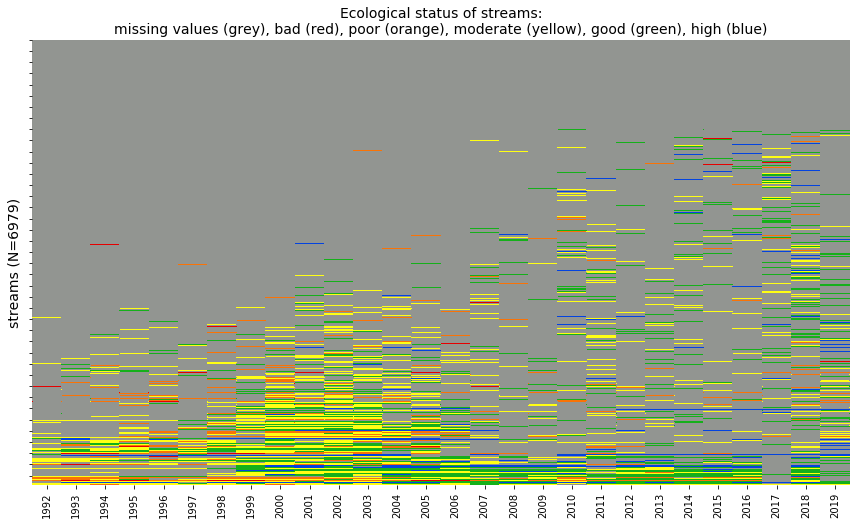
\includegraphics[width=\textwidth]{C:/Users/au687527/GitHub/GNNP/gis/output/missing_streams}
  \note{Heat map for each of the 7000 streams in VP2.\\\bigskip
  Grey indicates missing observations while a different color indicates the observed ecological status in a given year, i.e.
  \begin{itemize}
    \item Top: 9 \% of streams that has never been observed but still has a goal of achieving 'good' ecological status in VP2.
    \item Bottom: Streams observed most years.
    \item Throughout the 90s, $\frac{2}{3}$ of observations were poor/moderate.
    \item From 2009, majority of observations were good/high quality.
    \begin{itemize}
      \item Action Plan on the Aquatic Environment I (1987)
      \item Action Plan on the Aquatic Environment II (1998)
      \item Water Plan I (adopted by parliament 2009, municipal action plans 2010, measures came into effect 2012)
    \end{itemize}
  \end{itemize}
  }
\end{frame}

\begin{frame}
  \center
  \vspace{-1.4cm}
  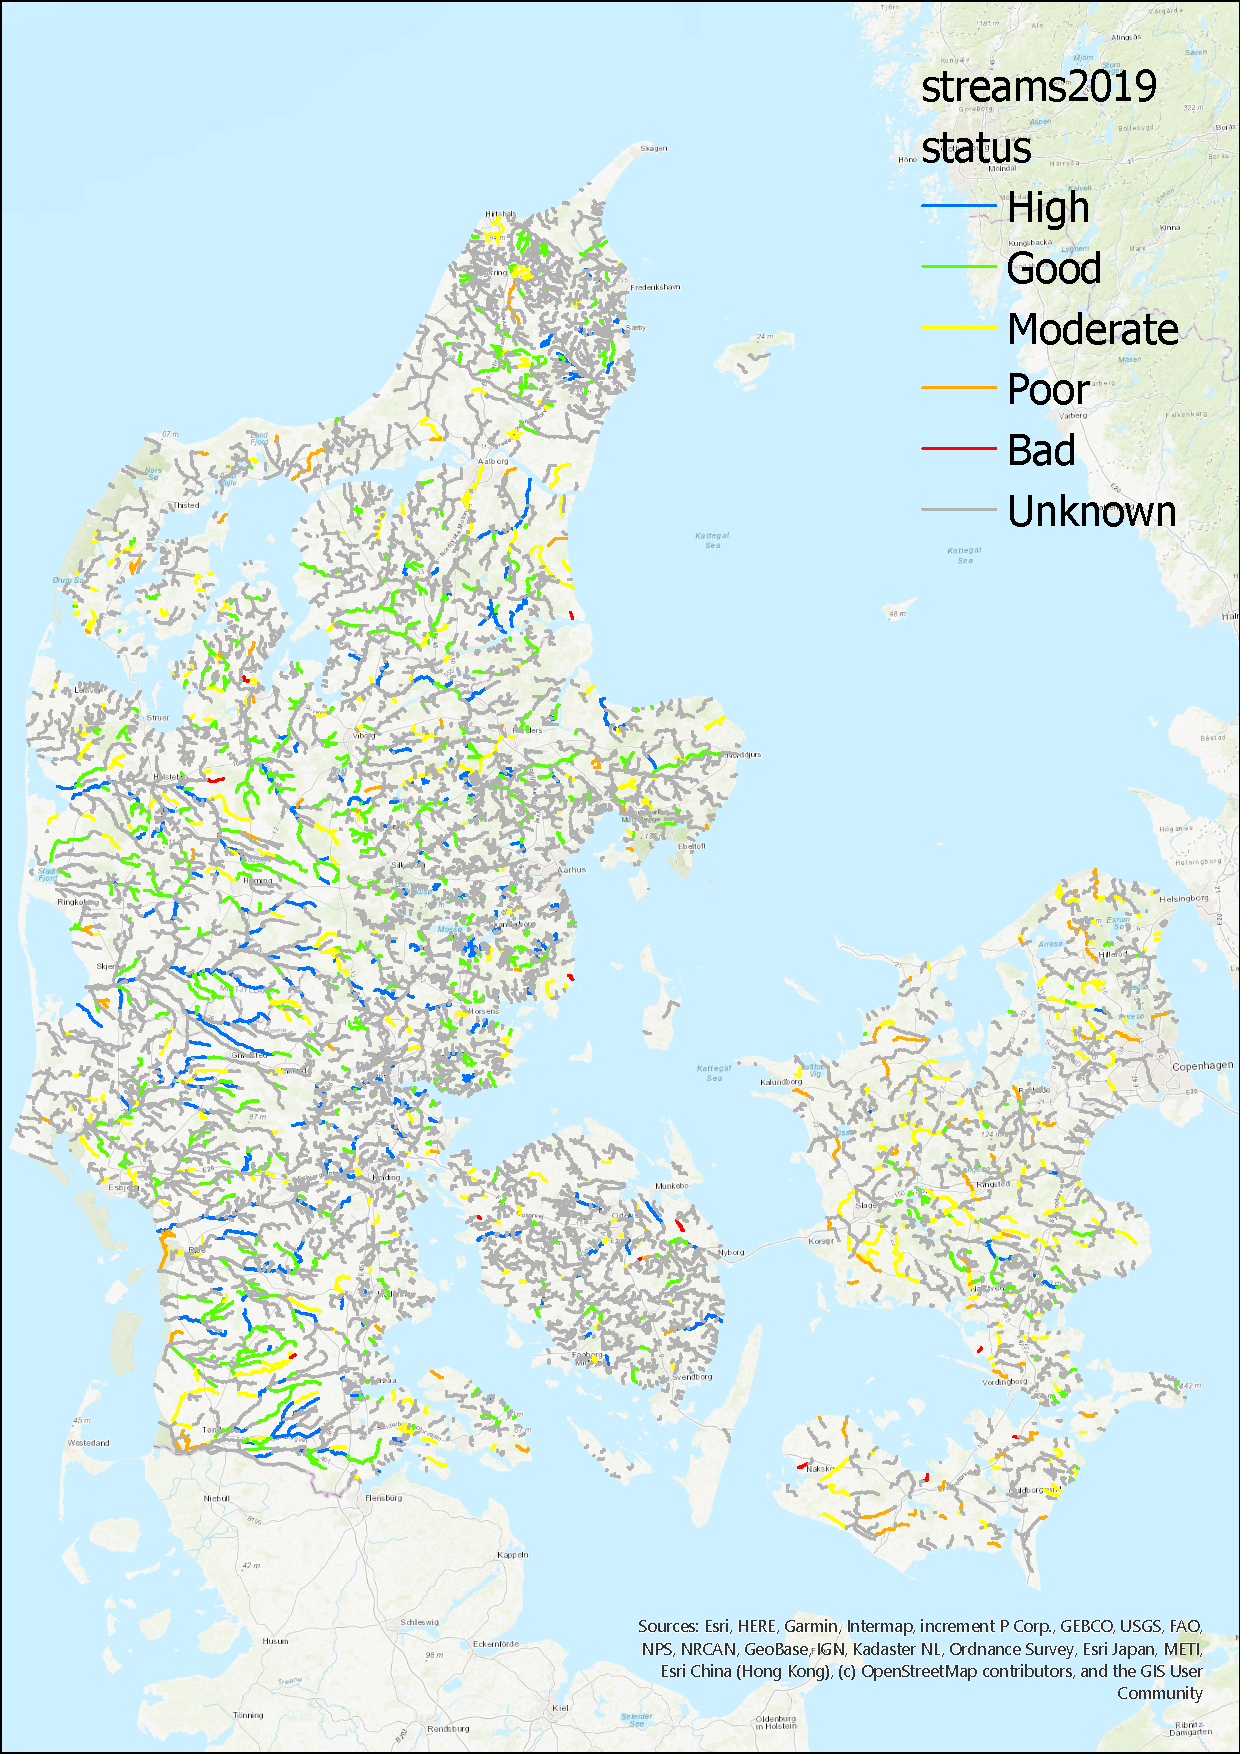
\includegraphics[width=.7\textwidth]{C:/Users/au687527/GitHub/GNNP/gis/output/streams2019}
  \note{In 2019, water quality is still mostly poor/moderate in Eastern DK.
  \\\bigskip
  On average, a quarter of the total stream length is assessed each year; grey lines represent unobserved streams.
  }
\end{frame}
\section{Apply valuation from stated preferences}

\begin{frame}{Apply valuation from stated preferences}\label<4>{frame:Valuation}
  The marginal willingness to pay using stated preference studies:
  \begin{itemize}
    \item \textbf{Surface waters}: Meta regressions analysis of 32 nordic studies \textcolor{grey}{(Zandersen, M., S. B. Olsen, L. Martinsen, T. E. Panduro, K. H. Zemo, and B. Hasler, 2022, DCE Scientific Report no. 486)}.
    \pause
    \item \textbf{Groundwater:} Choice experiment with 383 respondents around Limfjorden \textcolor{grey}{(Larsen, T. H., T. Lundhede, and S. B. Olsen, 2020, IFRO Working Paper)}. \hspace{4.5cm}\hyperlink{app:SurveyExample}{\beamerbutton{Questionnaire Example}}
    \pause
    \begin{itemize}\normalsize
      \item Overrepresentation of women and higher educated.
      \item WTP for improvement in groundwater quality from bad to good: 4,700 DKK (2019-prices).
    \end{itemize}
    \pause
    \item \textbf{Groundwater (old):} Choice experiment with 584 respondents \textcolor{grey}{(Hasler, B., T. Lundhede, L. Martinsen, S. Neye, and J. S. Schou, 2005, NERI Technical Report no. 543)}.
    \begin{itemize}\normalsize
      \item Exclusive focus on untreated vs treated drinking water.
      \item WTP for untreated drinking water: 987 DKK (2005-prices).
    \end{itemize}      
  \end{itemize}
  \note<1>{Shadow prices express the marginal current benefits of improving the quality of the Danish water environment on a national level. Measured as \textbf{(...)}
  }
  \note<2>{We have to rely on a single Danish study concerning the value of groundwater quality.
  }
  \note<3>{They find a substantial WTP which, however, might be slightly biased by overrepresentation of groups that often show higher WTP.
  }
  \note<4>{We acknowledge that there also exists an older study with a narrow focus on drinking water which we don't use.
  }
\end{frame}
\section{Growth decomposition}

\begin{frame}{Time series and decomposition of use value of water}
  Aggregate use value of all water environmental services depends on the number of households $N$ in catchment area $v$.\\\medskip
  Sum over all categories $\footnotesize l\in\{\text{groundwater, streams, lakes, coastal waters}\}$:
  \begin{align*}
    \mu_{u,t}^{w}W_t=\sum_v\sum_l\mu_{u,v,t}^{w,l}N_{v,t}
  \end{align*}
  \pause
  Contributors to growth in the real value of consumption of water environmental services from 1990-2020:
  \begin{itemize}
    \item Water quality \textcolor{darkgreen}{$\nearrow$}
    \item Age \textcolor{darkgreen}{$\nearrow$}
    \item Household income \textcolor{darkgreen}{$\nearrow$}
    \item Family patterns \textcolor{darkgreen}{$\nearrow$}
    \item Urbanization \textcolor{red}{$\searrow$}
  \end{itemize}
\end{frame}
\section{Takeaways}

\begin{frame}{Main takeaways}
  \begin{enumerate}
    \item Quality of the water environment improved from 1990-2020.
    \begin{itemize}
      \item If $\Delta\text{GNNI}>\Delta\text{NNI}\Rightarrow$ NNI and GDP underestimated growth.
    \end{itemize}
    \pause
    \item Changes in sociodemographic factors affect the Green NNI.
    \pause
    \item The marginal WTP per year for a water quality of \emph{good} as opposed to \emph{bad} would add up to:
    \begin{itemize}\normalsize
      \item DKK  7 b (2020-prices) for all streams.
      \item DKK  4 b (2020-prices) for all lakes.
      \item DKK  6 b (2020-prices) for all coastal waters.
      \item DKK 13 b (2020-prices) for all groundwater bodies.
    \end{itemize}
  \end{enumerate}
  \note<1>{\textbf{PRELIMINARY RESULTS AND DISCUSSION}\\
    Overall, the quality of ecosystem services has improved since 1990. That is likely to be offset by the costs of GHG emissions and the depletion of exhaustible natural resources\\
    - but if it should turn out that $\Delta\text{GNNI}>\Delta\text{NNP}$,
    \begin{itemize}
      \item[$\Rightarrow$] then it would indicate that GDP growth has not been at the expense of the environment according to the definition of "strong" sustainability.\\\bigskip
    \end{itemize}
    That is, with reservations that we don't fully live up to our international commitment such as the EU Water Framework Directive and the GHG reduction path implied by the Paris Agreement DESPITE outsourcing of our most polluting factories during the period.
  }
  % \note{\textbf{ROBUSTNESS}\\
  %   To construct an unbroken time series, we need to only rely on test methods for ecological and chemical quality that has been applied since the early 90s while applying so-called "heroic assumptions", thus
  %   \begin{itemize}
  %     \item[$\Rightarrow$] \textit{Comprehensive robustness checks are necessary}
  %   \end{itemize}
  %   some of which will have to be "back-of-the-envelope" calculations.
  % }
\end{frame}
% \begin{appendices}

% \begin{frame}{Appendix A: Imputation}
%   Imputation of missing observations:
%     \begin{itemize}
%       \item Estimated by \textit{multivariate imputation by chained equations (MICE)} where a \textit{fully conditional specification (FCS)} is constituted by a conditional density for each year.
%       \item Physical characteristics are included in a \textit{Bayesian ridge regression} using \textit{iteratively-reweighted regularized least-squares}.
%     \end{itemize}
  
%   \note{\textit{Our contributions are twofold.}\\\bigskip
%     \textbf{CONTRIBUTION 1}\\
%     \textbf{(...)} i.e. for all streams, lakes, fjords, coastal waters and groundwater bodies. DGP:
%     \begin{enumerate}
%       \item ... apply the conservative approach of using the observation that indicates the worst quality.
%       \item ... included in the latest Danish waterbody plan.
%       \item ... the reason is that data isn't representative but has a systematic overrepresentation of larger waterbodies and those of special concern for the ecological quality.
%       \item ... by estimating a linear trend and using it to predict.
%     \end{enumerate}
%   }
% \end{frame}

% \end{appendices}



\end{document}